\documentclass[parskip]{scrartcl}
\usepackage[utf8]{inputenc}
\usepackage[ngerman]{babel}
%\usepackage[round]{natbib}
%\usepackage{color} % used for comments
\usepackage[T1]{fontenc}

%Das Paket erzeugt ein anklickbares Verzeichnis in der PDF-Datei.
%\usepackage{hyperref}

%Das Paket wird für die anderthalb-zeiligen Zeilenabstand benötigt
\usepackage{setspace}

%%HTWM-Vorlage - benoetigt apt-get install texlive-fonts-extra
\setcounter{tocdepth}{3}				%Schatelungstiefe Inhaltsverz.
\usepackage[utf8]{inputenc}			%deutsche Umlaute
\usepackage{german, ngerman}
\usepackage[ngerman]{babel}			%Rechtschreibprüfung
\usepackage{color,listings} 			%Quellcode Highlighting, bindet das
\usepackage{float}					%% GRAFIKPOSITION MITTELS [H] ERWZINGEN
%Paket Listings ein
\usepackage{listings}
\usepackage{color}
\usepackage{textcomp}
\usepackage[T1]{fontenc}				%srccode
\usepackage[scaled]{beramono}		%srccode
\usepackage{longtable}				%mehrseitige tabellen
\usepackage[tableposition=b]{caption}
\usepackage[pdftex, pdftoolbar=false, hyperfootnotes=false, bookmarks,
bookmarksopen, bookmarksnumbered, bookmarksopenlevel=2, pdfpagelabels=true,
pdfstartpage=3, pdfstartview=FitH,]{hyperref} %Verlinkungen
\usepackage{array}					%farbige Tabellen
\usepackage[table]{xcolor} 			%farbige Tabellen
\usepackage{graphicx}				% \includegraphics bnoetigt dies

\usepackage{fancyhdr, graphicx}		%% Logo auf Titelseite
\renewcommand{\headrulewidth}{0pt}
\fancyhead[L]{}
\fancyhead[R]{
  \includegraphics[width=52mm]{./images/htwk.png}
}
%\usepackage{draftwatermark}			% wasserzeichen
	%Quelle: http://choorucode.com/2010/05/05/latex-adding-draft-watermark/?like=1&source=post_flair&_wpnonce=1c9f85538d
%\SetWatermarkText{VORABVERSION}		% wasserzeichen-text
%\SetWatermarkLightness{0.9}			% wasserzeichen-kontrast
%\SetWatermarkScale{2.5}				% wasserzeichen-zeichengroe\ss{}e

%%%% mathemathische Formeln zentrieren und vom Text absetzen mittels \[ E = mc^2 \] anstatt $ E = mc^2 $ %%%%
\usepackage{amsmath}
\usepackage{amsthm}
\usepackage{amsbsy}
\usepackage{amssymb}
%%%%%%%%%%%%%%%%%%%%%%%%%%%%%%%%%%%%%%%%%%%%%%%%%%%%%%%%%%%%%%%

\definecolor{Navy}{rgb}{0,0,0.5}
\definecolor{Gray}{gray}{0.5}
\definecolor{dunkelgrau}{rgb}{0.8,0.8,0.8}
\definecolor{hellgrau}{rgb}{0.95,0.95,0.95}
\definecolor{hellgrau2}{rgb}{0.93,0.93,0.93}

\hypersetup{
	colorlinks=true, 			% false: boxed links; true: colored links
	linkcolor=Navy,          		% color of internal links
	citecolor=Gray,        			% color of links to bibliography
	filecolor=magenta,      		% color of file links
	urlcolor=blue,           			% color of external links
	linkbordercolor={1 1 1}, 		% set to white
	citebordercolor={1 1 1} 		% set to white
}



\begin{document}
\subject{Projektdokumentation im Modul Semantic Web}
\title{Anzahl der Publikationen pro Mitarbiter der HTWK-Leipzig}
\author{Marcel Kirbst}
\date{\today}

\maketitle


\paragraph{Recherchefragestellung: }
Eine Liste aller Angestellten der HTWK-Leipzig, geordnet nach der Anzahl der bisherigen Publikationen im deutschsprachigen Raum.

\section{Inhaltliche Interpretation der Fragestellung}

Neben der Lehre stellt die Forschung und die Publikation deren Resultate eine wichtige Kernaufgabe der Professoren und wissenschaftlichen Mitarbeiter an Hochschulen dar. 
Die Aufgabe dieser Projektarbeit besteht daher zum einen darin, alle Mitarbeiter der HTWK-Leipzig zu ermitteln und in einer semantischen Datenbank zu erfassen. 

Weiterhin sind Daten aller im deutschsprachigen Raum erschienen Publikationen aufzubereiten und einzubinden. Diese Daten stellt die Deutsche Nationalbibliothek kostenfrei zur Verfügung.

Die Umsetzung des Projektes erfolgt auf einer virtuellen Maschine unter Verwendung der Virtualisierungslösung VirtualBox der Firma Oracle. Auf der virtuellen Maschine wurde als Gastbetriebssystem die Linux-Distribution Kubuntu 14.04 von Canonical eingesetzt. 

\section{Relevante Datenquellen}

An dieser Stelle erfolgt eine Auflistung aller relevanten Datenquellen und deren Beschreibung.

\subsection{Mitarbeiterkatalog der HTWK-Leipzig}

Die aktuellste, öffentlich zugängliche Auflistung aller Mitarbeiter der HTWK-Leipzig besteht aus dem HTWK-Telefonverzeichnis. Diese HTML-Seite lässt sich unter der Webadresse \cite{htwktel} abrufen.
Eine aufbereitete Version dieser Daten im JSON-Format wird von Herrn Henri Knochenhauer, B.Sc. und Herrn Roy Meisser, B.Sc unter \cite{htwkteljson} zur Verfügung gestellt und in diesem Projekt als Datenquelle genutzt.

\begin{tabular}{l|p{10cm}}
	Link & \url{http://141.57.21.45:8080/info/staff}\\
 	Datenformat & JSON \\
 	Schnittstelle & HTTP Rest-API \\
 	Lizenz & Daten: unbekannt. Datenquelle: GPL.\\
\end{tabular}

Die Daten dieser Datenquelle umfassen die eindeutige Mitarbeiteridentifikationsnummer, Nachname, Vornamen, akademischen Grad sowie die Fakultät jedes Mitarbeiters.


\subsection{Bibliothekskatalog der Deutsch Nationalbibliothek}

Die Deutsche Nationalbibliothek (DNB) sammelt alle deutschen Publikationen seit dem Jahr 1913. Darüber hinaus bietet sie umfangreiche Dienstleistungen für Bibliotheken und Wissenschaftler an. Mittels einer durch die DNB vergebenen Normdatensatz (GND)\footnote{Gemeinsame Normdatei} lassen sich Werke, Personen oder Körperschaften identifizieren. Diese Identifizierung ermöglicht es Personen unterschiedlicher Quellen zu verlinken.

\begin{tabular}{l|p{10cm}}
	Link & \url{http://datendienst.dnb.de/cgi-bin/mabit.pl?userID=opendata&pass=opendata&cmd=login} \\
 	Datenformat & RDF \\
 	Schnittstelle & Linked Data, Dump, Rest-API \\
 	Lizenz & CC-SA \\
\end{tabular}

Die Daten lassen sich unter der angegebenen Webadresse direkt herunterladen. Für dieses Projekt wurde die Datei GND.rdf.gz herunter geladen, welche die gesammelten Normdaten zu den Autoren enthält und entpackt derzeit etwa 9 GByte groß ist
Weiterhin wurde die Datei DNBTitel.rdf.gz heruntergeladen. Diese Datei enthält die Namen und Autoren aller Werke der Deutschen Nationalbibliothek und ist entpackt derzeit etwa 12 GByte groß. 

\section{Extraktion relevanter Daten und import in einen Triplestore }

Die Extraktion aller 3 Dateien erfolgt über eine für dieses Projekt erstellte JAVA-Anwendung, welche im Repository zu diesem Projekt hinterlegt ist. Das Repository kann unter folgender Webadresse abgerufen werden\cite{gitmkirbstsm}.

\subsection{Extraktion der HTWK-Mitarbeiter}
Die Daten der HTWK-Mitarbeiter liegen im JSON Format vor. Die exakte Struktur zeigt das folgende Listing auszugsweise. 

\definecolor{listinggray}{gray}{0.9}
\definecolor{lbcolor}{rgb}{0.9,0.9,0.9}
\lstset{
	language=XML,
	keywordstyle=\bfseries\ttfamily\color[rgb]{0,0,1},
	identifierstyle=\ttfamily,
	commentstyle=\color[rgb]{0.133,0.545,0.133},
	stringstyle=\ttfamily\color[rgb]{0.627,0.126,0.941},
	showstringspaces=false,
	basicstyle=\scriptsize,
	numbers=left,
	stepnumber=1,
	numbersep=6pt,
	numberstyle=\tiny,
	tabsize=1,
	breaklines=true,	%automatischer Zeilenumbruch
	prebreak = \raisebox{0ex}[0ex][0ex]{\ensuremath{\hookleftarrow}},
	breakatwhitespace=false,
	aboveskip={1.5\baselineskip},
  	columns=fixed,
  	upquote=true,
  	extendedchars=true,
  	backgroundcolor=\color[rgb]{0.97,0.97,0.97},
}
\begin{lstlisting}[captionpos=b, caption=Format der importierten HTWK-Mitarbeiterdaten, label=Format der importierten HTWK-Mitarbeiterdaten]
[
  - {
     cuid: "597",
     name: "Siebeck, Andrea",
     degree: "Dipl.-Angl.",
     faculty: "AAA"
  },
  - {
  {
     cuid: "8",
     name: "Engel, Heike",
     degree: "Dipl.-Wirtschaftsinf.",
     faculty: "DF"
  }
]
\end{lstlisting}

Die JAVA-Anwendung bezieht das JSON-Dokument direkt von der Webressource. Die JAVA-Anwendung generiert aus den importierten Daten eine RDF-Datei, welche nach folgendem RDF-Schema generiert wird.
\definecolor{listinggray}{gray}{0.9}
\definecolor{lbcolor}{rgb}{0.9,0.9,0.9}
\lstset{
	language=XSLT,
	keywordstyle=\bfseries\ttfamily\color[rgb]{0,0,1},
	identifierstyle=\ttfamily,
	commentstyle=\color[rgb]{0.133,0.545,0.133},
	stringstyle=\ttfamily\color[rgb]{0.627,0.126,0.941},
	showstringspaces=false,
	basicstyle=\scriptsize,
	numbers=left,
	stepnumber=1,
	numbersep=6pt,
	numberstyle=\tiny,
	tabsize=1,
	breaklines=true,	%automatischer Zeilenumbruch
	prebreak = \raisebox{0ex}[0ex][0ex]{\ensuremath{\hookleftarrow}},
	breakatwhitespace=false,
	aboveskip={1.5\baselineskip},
  	columns=fixed,
  	upquote=true,
  	extendedchars=true,
  	backgroundcolor=\color[rgb]{0.97,0.97,0.97},
}
\begin{lstlisting}[captionpos=b, caption=RDF-Schema der exportierten HTWK-Mitarbeiterdaten, label=RDF-Schema der exportierten HTWK-Mitarbeiterdaten]
@prefix rdf: <http://www.w3.org/1999/02/22-rdf-syntax-ns#> .
@prefix rdfs: <http://www.w3.org/2000/01/rdf-schema#> .
@prefix owl: <http://www.w3.org/2002/07/owl#> .
@prefix xsd: <http://www.w3.org/2001/XMLSchema#> .
@prefix : <https://raw.githubusercontent.com/mkirbst/semanticweb/master/scheme#> .
 
:Employee a rdfs:Class .
:Publications a rdfs:Class .

:Int a rdfs:Datatype; owl:onDatatype  xsd:integer; xsd:minInclusive 1 .
:String a rdfs:Datatype; owl:onDatatype  xsd:string .
 
:cuid a rdf:Property; rdfs:domain :Employee; rdfs:range :Int .
:lastname a rdf:Property; rdfs:domain :Employee; rdfs:range :String .
:firstname a rdf:Property; rdfs:domain :Employee; rdfs:range :String .
:degree a rdf:Property; rdfs:domain :Employee; rdfs:range :String .
:dnbautorid a rdf:Property; rdfs:domain :Employee; rdfs:range :Int .
:birth a rdf:Property; rdfs:domain :Employee; rdfs:range :Int .
 
:dnbpubid a rdf:Property; rdfs:domain :Publication; rdfs:range :Int .
:dnbautorid a rdf:Property; rdfs:domain :Publication; rdfs:range :Int .
:title a rdf:Property; rdfs:domain :Publication; rdfs:range :String .
:pubdate a rdf:Property; rdfs:domain :Publication; rdfs:range :Int .
\end{lstlisting}

Da diese Datei im Format N3 vorliegt, wurde diese mit einem RDF-Translator \cite{rdftransformator} in das XML-Format überführt.

Die vom Java-Programm generierte RDF-Datei kann nun direkt über die Webschnittstelle in OntoWiki importiert werden und hat folgendes Format.
\definecolor{listinggray}{gray}{0.9}
\definecolor{lbcolor}{rgb}{0.9,0.9,0.9}
\lstset{
	language=XSLT,
	keywordstyle=\bfseries\ttfamily\color[rgb]{0,0,1},
	identifierstyle=\ttfamily,
	commentstyle=\color[rgb]{0.133,0.545,0.133},
	stringstyle=\ttfamily\color[rgb]{0.627,0.126,0.941},
	showstringspaces=false,
	basicstyle=\scriptsize,
	numbers=left,
	stepnumber=1,
	numbersep=6pt,
	numberstyle=\tiny,
	tabsize=1,
	breaklines=true,	%automatischer Zeilenumbruch
	prebreak = \raisebox{0ex}[0ex][0ex]{\ensuremath{\hookleftarrow}},
	breakatwhitespace=false,
	aboveskip={1.5\baselineskip},
  	columns=fixed,
  	upquote=true,
  	extendedchars=true,
  	backgroundcolor=\color[rgb]{0.97,0.97,0.97},
}
\begin{lstlisting}[captionpos=b, caption=RDF-Format der exportierten HTWK-Mitarbeiterdaten, label=RDF-Format der exportierten HTWK-Mitarbeiterdaten]
<rdf:RDF
  xmlns:semweb="https://raw.githubusercontent.com/mkirbst/semanticweb/master/scheme#"
  xmlns:rdf="http://www.w3.org/1999/02/22-rdf-syntax-ns#"
>

  <semweb:Employee rdf:about="https://raw.githubusercontent.com/mkirbst/semanticweb/master/htwkstaff.json#cuid597">
    <semweb:cuid>597</semweb:cuid>
    <semweb:lastname>Siebeck</semweb:lastname>
    <semweb:firstname> Andrea</semweb:firstname>
    <semweb:degree>Dipl.-Angl.</semweb:degree>
    <semweb:faculty>AAA</semweb:faculty>
    <semweb:dnbautorid>0</semweb:dnbautorid>
    <semweb:birth>0</semweb:birth>
  </semweb:Employee>
  <semweb:Employee rdf:about="https://raw.githubusercontent.com/mkirbst/semanticweb/master/htwkstaff.json#cuid8">
    <semweb:cuid>8</semweb:cuid>
    <semweb:lastname>Engel</semweb:lastname>
    <semweb:firstname> Heike</semweb:firstname>
    <semweb:degree>Dipl.-Wirtschaftsinf.</semweb:degree>
    <semweb:faculty>DF</semweb:faculty>
    <semweb:dnbautorid>0</semweb:dnbautorid>
    <semweb:birth>0</semweb:birth>
  </semweb:Employee>
</rdf:RDF>
\end{lstlisting}

\subsection{Extraktion der Daten der Deutschen Nationalbibliothek}
Unter der Webadresse \cite{dnbdata} lassen sich die benötigten Daten direkt im RDF-Format herunterladen. Die heruntergeladenen Dateien sind jedoch mit 9 und 12 GByte so groß,
das diese nicht direkt über die Webschnittstelle des OntoWiki importiert werden können. 

Aus diesem Grund filtert die JAVA-Anwendung aus den Datensätzen nur diese heraus, deren Autor den Vor- und Nachname von HTWK-Mitarbeitern enthält. Um diese Operationen effizient durchführen zu können, werden in der JAVA-Anwendung Hashmaps erzeugt, die als Schlüssel die betreffenden RDF-Tags so wie Vor- und Nachname als Hashwert enthalten. Durch diese Implementierungsvariante werden die Vorteile der Hashmap-Datenstruktur genutzt. Außerdem werden so wenig wie möglich rechenintensive Stringmanipulationen durchgeführt. 

\definecolor{listinggray}{gray}{0.9}
\definecolor{lbcolor}{rgb}{0.9,0.9,0.9}
\lstset{
	language=Java,
	keywordstyle=\bfseries\ttfamily\color[rgb]{0,0,1},
	identifierstyle=\ttfamily,
	commentstyle=\color[rgb]{0.133,0.545,0.133},
	stringstyle=\ttfamily\color[rgb]{0.627,0.126,0.941},
	showstringspaces=false,
	basicstyle=\scriptsize,
	numbers=left,
	stepnumber=1,
	firstnumber=199,
	numbersep=6pt,
	numberstyle=\tiny,
	tabsize=1,
	breaklines=true,	%automatischer Zeilenumbruch
	prebreak = \raisebox{0ex}[0ex][0ex]{\ensuremath{\hookleftarrow}},
	breakatwhitespace=false,
	aboveskip={1.5\baselineskip},
  	columns=fixed,
  	upquote=true,
  	extendedchars=true,
  	backgroundcolor=\color[rgb]{0.97,0.97,0.97},
}
\begin{lstlisting}[captionpos=b, caption=Auszug JAVA-Anwendung: Hashmap zur schnelleren Filterung der Normdaten, label=Auszug JAVA-Anwendung: Hashmap zur schnelleren Filterung der Normdaten]
Map<String, emp>hEmps = new HashMap<String, emp>();
\end{lstlisting}

\lstset{
	language=Java,
	keywordstyle=\bfseries\ttfamily\color[rgb]{0,0,1},
	identifierstyle=\ttfamily,
	commentstyle=\color[rgb]{0.133,0.545,0.133},
	stringstyle=\ttfamily\color[rgb]{0.627,0.126,0.941},
	showstringspaces=false,
	basicstyle=\scriptsize,
	numbers=left,
	stepnumber=1,
	firstnumber=233,
	numbersep=6pt,
	numberstyle=\tiny,
	tabsize=1,
	breaklines=true,	%automatischer Zeilenumbruch
	prebreak = \raisebox{0ex}[0ex][0ex]{\ensuremath{\hookleftarrow}},
	breakatwhitespace=false,
	aboveskip={1.5\baselineskip},
  	columns=fixed,
  	upquote=true,
  	extendedchars=true,
  	backgroundcolor=\color[rgb]{0.97,0.97,0.97},
}
\begin{lstlisting}[captionpos=b, caption=Auszug JAVA-Anwendung: Einfügen von Objekten in die Hashmap, label=Auszug JAVA-Anwendung: Einfügen in die Hashmap]
//DNB-GND.rdf name format as hasmap key value
hEmps.put("<rdf:li>"+name+"</rdf:li>", tmpemp);
\end{lstlisting}


\definecolor{listinggray}{gray}{0.9}
\definecolor{lbcolor}{rgb}{0.9,0.9,0.9}
\lstset{
	language=Java,
	keywordstyle=\bfseries\ttfamily\color[rgb]{0,0,1},
	identifierstyle=\ttfamily,
	commentstyle=\color[rgb]{0.133,0.545,0.133},
	stringstyle=\ttfamily\color[rgb]{0.627,0.126,0.941},
	showstringspaces=false,
	basicstyle=\scriptsize,
	numbers=left,
	stepnumber=1,
	firstnumber=135,
	numbersep=6pt,
	numberstyle=\tiny,
	tabsize=1,
	breaklines=true,	%automatischer Zeilenumbruch
	prebreak = \raisebox{0ex}[0ex][0ex]{\ensuremath{\hookleftarrow}},
	breakatwhitespace=false,
	aboveskip={1.5\baselineskip},
  	columns=fixed,
  	upquote=true,
  	extendedchars=true,
  	backgroundcolor=\color[rgb]{0.97,0.97,0.97},
}
\begin{lstlisting}[captionpos=b, caption=Auszug JAVA-Anwendung: RDF-Parser , label=Auszug JAVA-Anwendung RDF-Parser]
	int hits = 0;
	String begintag = "<rdf:Description";
	String endtag = "</rdf:Description";
	String nametag = "<gndo:preferredNameForThePerson>";
	StringBuilder t3 = new StringBuilder();
	String ts3 = "";
	boolean found = false;

	BufferedReader br = new BufferedReader(new FileReader(gndfilepath));
	String line;

	while ((line = br.readLine()) != null) {
		String linetrimmed = line.trim();	// performance: trim only once
		
		//linetrimmed begins with begintag OR nametag OR endtag OR other 
		if(linetrimmed.startsWith(begintag)) 
		{			
			t3 = new StringBuilder();
			t3.append(line+"\n");
			found = false;
		} else if (linetrimmed.startsWith(nametag)) 
		{
			t3.append(line+"\n");
			if(hEmps.containsKey(linetrimmed)) {  //hEmps == hashmap containing htwk employee objects
				found = true;
				hits++;
			}
		} else if (linetrimmed.startsWith(endtag)) {
			t3.append(line+"\n\n");
			if(found == true)  {
				System.out.println(hits + " " + t3.toString());
				writer.write(t3.toString());
			}
		} else {
			t3.append(line+"\n");
		}
	}
\end{lstlisting}

Das resultierende JAVA-Programm verarbeitet die gesamten Datensätze beider Dateien innerhalb einer Laufzeit von circa 2 Minuten. Die zu Grunde liegende Hardware ist eine Laptop der Marke HP EliteBook 8470w (CPU:Intel(R) Core(TM) i7-3740QM CPU @ 2.70GHz, RAM 16 GB, Primärspeicher: Micron SSD 250 GB ).

Die resultierenden beiden Dateien haben exakt das gleiche RDF-Format wie die Eingabedateien, jedoch bereinigt um alle Datensätze, deren Autoren nicht einen Namen eines HTWK-Mitarbeiters tragen. Diese Dateien lassen sich nun über die Webschnittstelle von OntoWiki importieren.

\section{Verlinkung von Ressourcen}

Mit den 3 verwendeten Datenquellen lassen sich die Daten auf 2 Arten verknüpfen um die gewünschten Ergebnisse zu erhalten. Die Daten der Deutschen Nationalbibliothek sehen für jeden Autor eine eindeutige Identifikationsnummer vor. Als problematisch haben sich im Verlauf des Projektes dabei 2 Umstände erwiesen. 

Die Deutsche Nationalbibliothek weist darauf hin das sich die für das Projekt verwendeten Daten noch in einem Migrationsprozess befinden und noch nicht vollständig konsistent sind. Daraus resultiert, dass manche Autoren mehrfach mit unterschiedlichen Publikationen im Datenbestand vorhanden sind. 

Das zweite Problem besteht darin, dass von der Datenquelle HTWK-Telefonbuch nur Nachname und Vornamen für die Verlinkung einbezogen werden können. Weitere hilfreiche Attribute wie beispielsweise das Geburtsjahr sind in dieser Datenquelle nicht hinterlegt. Für ein wirklich tragfähiges Ergebnis des Projekts sollten folglich konsistente Datenquellen heran gezogen werden.

\section{Anfrage an die Forschungswissensbasis}

\subsection{SPARQL-Anfrage}

\lstset{
	language=SQL,
	 morekeywords={PREFIX},
	keywordstyle=\bfseries\ttfamily\color[rgb]{0,0,1},
	identifierstyle=\ttfamily,
	commentstyle=\color[rgb]{0.133,0.545,0.133},
	stringstyle=\ttfamily\color[rgb]{0.627,0.126,0.941},
	showstringspaces=false,
	basicstyle=\scriptsize,
	numbers=left,
	stepnumber=1,
	firstnumber=1,
	numbersep=6pt,
	numberstyle=\tiny,
	tabsize=1,
	breaklines=true,	%automatischer Zeilenumbruch
	prebreak = \raisebox{0ex}[0ex][0ex]{\ensuremath{\hookleftarrow}},
	breakatwhitespace=false,
	aboveskip={1.5\baselineskip},
  	columns=fixed,
  	upquote=true,
  	extendedchars=true,
  	backgroundcolor=\color[rgb]{0.97,0.97,0.97},
}
\begin{lstlisting}[captionpos=b, caption=SPARQL-Abfrage, label=SPARQL-Abfrage]
PREFIX bibo: <http://purl.org/ontology/bibo/>
PREFIX ns3: <http://purl.org/ontology/bibo/>
PREFIX owl: <http://www.w3.org/2002/07/owl#>
PREFIX xsd: <http://www.w3.org/2001/XMLSchema#>
PREFIX ns2: <http://rdvocab.info/>
PREFIX dct: <http://purl.org/dc/terms/>
PREFIX dc: <http://purl.org/dc/elements/1.1/>
PREFIX ns1: <http://iflastandards.info/ns/isbd/elements/>
PREFIX ns0: <http://id.loc.gov/vocabulary/relators/>
PREFIX semweb: <https://raw.githubusercontent.com/mkirbst/semanticweb/master/scheme#>
PREFIX rdf: <http://www.w3.org/1999/02/22-rdf-syntax-ns#>
PREFIX marcRole: <http://id.loc.gov/vocabulary/relators/>

select ?person ?lastname ?firstname (count(?document)+count(?article) as ?count)
where {
  ?person rdf:type semweb:Employee;
          semweb:lastname ?lastname;
          semweb:firstname ?firstname .
  
  ?document rdf:type ns3:Document;
            marcRole:edt ?editor .
  
  ?article rdf:type bibo:Article;
            marcRole:edt ?aeditor;
            dc:creator ?acreator
  
  Filter ( 
    strstarts(concat(?editor, ""), ?lastname)
    AND strends(concat(?editor, ""), ?firstname)
    AND strstarts(concat(?aeditor, ""), ?lastname)
    AND strends(concat(?aeditor, ""), ?firstname)
    
  )
  }
LIMIT 200
\end{lstlisting}

\clearpage
\subsection{Ergebnis der Anfrage}

\begin{figure}[htb]
\begin{center}
 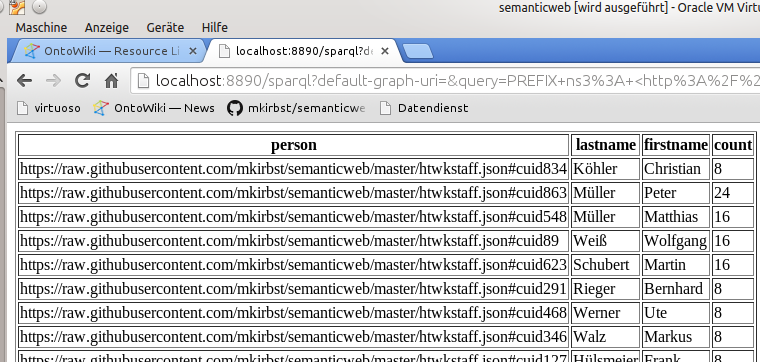
\includegraphics[width=1\hsize]{./images/querryresult.png}
 \end{center}
\caption[Ergebnis der SPARQL-Abfrage]{\label{querryresult}Ergebnis der SPARQL-Abfrage}
\end{figure}

\section{Interpretation und Zusammenfassung}
Zusammenfassend lässt sich feststellen das die semantische Verknüpfung der Daten auf diese Weise möglich ist. Mit dem derzeitigen Datenbestand lassen sich jedoch automatisiert keine zufriedenstellenden Resultate erzielen.
Sollten die zu Grunde liegenden Daten der Deutschen Nationalbibliothek in Zukunft in einem vollständig konsistenten Zustand befinden, ist mit aussagekräftigeren Ergebnissen zu rechnen. Ein manueller Abgleich der einzelnen Personendaten oder die Zuhilfename weiterer
Autoreneigenschaften, wie beispielsweise des Geburtsdatums lassen ebenfalls eine höhere Qualität der Ergebnisse erwarten.

Alle Ressourcen zu diesem Projekt sind im Repository unter der Webadresse \cite{gitmkirbstsm} hinterlegt.

%\bibliographystyle{lnig.bst}
%\bibliography{Projektdokumentation}

\clearpage
\renewcommand\refname{Projektdokumentation}
\begin{thebibliography}{999}

\bibitem{htwktel}    
\url{http://www.htwk-leipzig.de/de/hochschule/telefonverzeichnis/}\\
abrufbar am 11.06.2014

\bibitem{htwkteljson}
\url{http://141.57.21.45:8080/info/staff}
abrufbar am 22.06.2014

\bibitem{gitmkirbstsm}    
\url{https://github.com/mkirbst/semanticweb}\\
abrufbar am 12.06.2014


\bibitem{rdftransformator}    
\url{http://rdf-translator.appspot.com/}\\
abrufbar am 25.06.2014


\bibitem{dnbdata}    
\url{http://datendienst.dnb.de/cgi-bin/mabit.pl?userID=opendata&pass=opendata&cmd=login}\\
abrufbar am 25.06.2014

\end{thebibliography}

\end{document}
